\documentclass[a4paper]{ctexart}
\usepackage{xeCJK}
\usepackage{amsmath}
\usepackage{amssymb}
\usepackage{bm}
\usepackage{graphicx}
\usepackage[linesnumbered,ruled,lined]{algorithm2e}
\newcommand{\code}[1]{{\texttt{#1}}}

\usepackage{pdfpages}

\usepackage{pgf}
\usepackage{tikz}
\usetikzlibrary{arrows, decorations.pathmorphing, backgrounds, positioning, fit, petri, automata}


% Title
\title{《算法设计与分析》2018期末考试真题}
\author{尹达恒}
\date{2020/12/21}
 
\begin{document}

\begin{titlepage}
\maketitle
\end{titlepage}
\includepdfmerge{2018秋算法试卷.pdf,1-2}

% !TeX root = ./homework.tex
\section{题解2}
\subsection{问题分析}
最长公共子串问题是一个典型的动态规划问题,最长公共子序列在删去最后一个公共字符后,仍然是剩下字符串的最长公共子序列,因此可得如下递推公式:
$$
C[i,j]=\left\{
\begin{aligned}
    max\{C[i-1,j],C[i,j-1]\}&\quad&(A[i]=B[j])\\
    C[i-1,j-1]+1\}&&(A[i]\not =B[j])\\
\end{aligned}
\right.
$$

\subsection{算法伪代码}
见算法\ref{alg:2}。
\begin{algorithm}[htbp]
\caption{题解2算法伪代码}\label{alg:2}
\SetKwProg{Fn}{Function}{ begin}{end}
\Fn{F($S$)}{
    \KwIn{字符串$A,B$}
    \KwOut{最长公共子串长度$C$}
    \leIf{$A[i]=B[j]$}{$C[1,1]=1$}{$C[1,1]=0$}
    \For{$i\in[2,m]$}{
        \For{$j\in[2,n]$}{
            $$
            C[i,j]=\left\{
            \begin{aligned}
                max\{C[i-1,j],C[i,j-1]\}&\quad&(A[i]=B[j])\\
                C[i-1,j-1]+1\}&&(A[i]\not =B[j])\\
            \end{aligned}
            \right.
            $$
        }
    }
    \Return $C[m,n]$\;
}
\end{algorithm}
% !TeX root = ./homework.tex
\section{题解3}
\subsection{问题a}
将坐标点按横坐标排序,选出左边的$\lfloor\frac{n}{2}\rfloor$个点为一部分,剩下的为第二部分。

\subsection{问题b}
\begin{figure}[htbp]
    \centering
    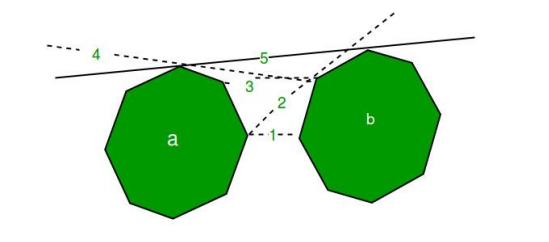
\includegraphics[width=1\textwidth]{截图.png}
    \caption{示意图}
\end{figure}
查找合并凸包的上方连线时,从左边部分的最右点和右边部分的最左点连线开始查找:
\begin{enumerate}
    \item 固定右边的点,遍历左凸包上在连线上方的点
    \item 找到与原连线夹角最大的新连线
    \item 固定左边的点,遍历右凸包上在连线上方的点
    \item 找到与原连线夹角最大的新连线
    \item 重复直到找不到新连线
\end{enumerate}
查找合并凸包的下方连线时,从左边部分的最右点和右边部分的最左点连线开始查找:
\begin{enumerate}
    \item 固定右边的点,遍历左凸包上在连线下方的点
    \item 找到与原连线夹角最大的新连线
    \item 固定左边的点,遍历右凸包上在连线下方的点
    \item 找到与原连线夹角最大的新连线
    \item 重复直到找不到新连线
\end{enumerate}

\subsection{问题c}
算法的主要时间都花在将小凸包合并为大凸包的过程上。
% !TeX root = ./homework.tex
\section{题解4}
\subsection{问题分析}
显然,本题的贪心选择性是:每个小朋友$p_i$都只要选择能与自己匹配的最大的$p_j$即可。

可以通过反证法证明此方法最优:如果对于某个配对$p_i,p_j$,存在一个$p_k<p_j$,使$p_i$不与$p_j$配对而与$p_k$配对时,能增加一个配对$p_j,p_l$,如果要这种情况成立,那么必然有:
$$
\left\{
\begin{aligned}
    p_i+p_j\leq B\\
    p_k<p_j\\
    p_i+p_k\leq B\\
    p_k+p_l>B\\
    p_j+p_l\leq B\\
\end{aligned}
\right.
$$
但显然,$p_j+p_l>p_k+p_l>B$,不可能有$p_j+p_l\leq B$,因此此方法不是最优的情况不存在。

\subsection{算法伪代码}
见算法\ref{alg:4}。
\begin{algorithm}[htbp]
\caption{题解4算法伪代码}\label{alg:4}
\SetKwProg{Fn}{Function}{ begin}{end}
\Fn{F($p_i$)}{
    \KwIn{小朋友的数字牌$\{p_i\}$、匹配和限制$B$}
    \KwOut{能匹配的最多对小朋友$C$}
    对$\{p_i\}$进行排序\;
    \Repeat{$\{p_i\}$中只剩1个或0个元素}{
        选出$\{p_i\}$中最大的元素$p$\;
        从$\{p_i\}$中删去$p$\;
        \lIf{$p\geq B$}{continue}
        选出$\{p_i\}$中$\leq B-p$最大的元素$p'$\;
        从$\{p_i\}$中删去$p'$\;
        $C=C+1$\;
    }
    \Return{$C$}
}
\end{algorithm}
% !TeX root = ./homework.tex
\section{题解5}
\subsection{问题分析}
此问题可以通过分治求解,对于上部的焊点$T_i$和下部的焊点$B_i$,可以通过如下方式求它们的相交次数:
\begin{itemize}
    \item 分治:分别递归地计算$T_i,i\in[1,n/2]$和$T_i,i\in[n/2+1]$的相交点个数,并对$T_i,i\in[1,n/2]$和$T_i,i\in[n/2+1]$所连接的下部焊点编号进行排序
    \item 组合:对于$T_i,i\in[1,n/2]$,将其对应的上部焊点编号与$T_i,i\in[n/2+1]$对应的上部焊点编号比较,$T_i,i\in[1,n/2]$上部编号较大的与$T_i,i\in[n/2+1]$上部编号较小的相交,求出相交数量;对于$T_i,i\in[n/2+1]$同理。最终求出相交点数之和即最终结果。
\end{itemize}

\subsection{算法伪代码}
见算法\ref{alg:5}。
\begin{algorithm}[htbp]
\caption{题解5算法伪代码}\label{alg:5}
\SetKwProg{Fn}{Function}{ begin}{end}
\Fn{$F(T)$}{
    \KwIn{上部焊点对应的下部焊点编号$T$,$T_i=j$表示上部焊点$i$与下部焊点$j$相连}
    \KwOut{相交焊点数$S$,所有的下部焊点编号排序结果$B$}
    $S_1,B_1=F(\{T_i|i\in[1,|T|/2]\})$\;
    $S_2,B_2=F(\{T_i|i\in[|T|/2+1,|T|]\})$\;
    $S=S_1+S_2$\;
    $B=\{\},k=1,t=0$\;
    \Repeat{}{
        \eIf{$B_1[i]>B_2[j]$}{
            $B[k]=B_2[j]$\;
            $j=j+1$\;
            $t=t+1$\;
        }{
            $B[k]=B_1[i]$\;
            $i=i+1$\;
            $S=S+t$\;
            $t=j-1$\;
        }
        $k=k+1$\;
    }
    \Return $S,B$
}
\end{algorithm}
% !TeX root = ./homework.tex
\section{题解6}
\subsection{问题分析}
显然,对于$n$个点,它们的间距有$n-1$个,将其组织为一个数组$A$,原覆盖问题就可以看作选择这个数组中的连续几个值,显然,总共有$(n-1)+(n-2)+\dots+2+1=n(n-1)/2$种选法遍历所有这些选法就能得到$O(n^2)$时间的算法。

但实际上这$n(n-1)/2$种选法并不需要全部遍历,可以从第一个间距开始增加,如果长度超过绳长度,就将开头处的距离减去,直到增加到最后一个间距,时间复杂度为$O(n)$。

\subsection{算法伪代码}
$O(n^2)$时间的算法见算法\ref{alg:6-1}。
\begin{algorithm}[htbp]
\caption{题解6算法伪代码}\label{alg:6-1}
\SetKwProg{Fn}{Function}{ begin}{end}
\Fn{$F(T)$}{
    \KwIn{点的间距列表$A$,绳子长度$L$}
    \KwOut{覆盖的最大点数$m$}
    $m=0$\;
    \For{$i\in [1,|A|]$}{
        $S=0,k=1$\;
        \For{$j\in [i,|A|]$}{
            $S=S+A[j]$\;
            $k=k+1$\;
            \If{$S<=L\wedge k>m$}{
                $m=k$\;
            }
        }
    }
    \Return $m$
}
\end{algorithm}
$O(n)$时间的算法见算法\ref{alg:6-2}。
\begin{algorithm}[htbp]
\caption{题解6算法伪代码}\label{alg:6-2}
\SetKwProg{Fn}{Function}{ begin}{end}
\Fn{$F(T)$}{
    \KwIn{点的间距列表$A$,绳子长度$L$}
    \KwOut{覆盖的最大点数$m$}
    $m=0$\;
    \For{$i\in [1,|A|]$}{
        $S=0,k=1$\;
        \For{$j\in [i,|A|]$}{
            $S=S+A[j]$\;
            $k=k+1$\;
            \If{$S>L$}{
                break\;
            }
            \If{$S<=L\wedge k>m$}{
                $m=k$\;
            }
        }
    }
    \Return $m$
}
\end{algorithm}
% !TeX root = ./homework.tex
\section{题解7}
\subsection{问题分析}
此问题可以是典型的动态规划问题。对于物品$a_i$和剩余$C_1$、$C_2$、$C_3$的三个背包,背包方案的最优解必然是下面三个中价值最大的那个:
\begin{itemize}
    \item 物品$a_i$不放入任何背包,$C_1$、$C_2$、$C_3$中装入剩下的物品
    \item 物品$a_i$放入背包1,$C_1-w_i$、$C_2$、$C_3$中装入剩下的物品
    \item 物品$a_i$放入背包2,$C_1$、$C_2-w_i$、$C_3$中装入剩下的物品
    \item 物品$a_i$放入背包3,$C_1$、$C_2$、$C_3-w_i$中装入剩下的物品
\end{itemize}
由此可得最优解$M(i,C_1,C_2,C_3),i\in [1,n]$的递推关系式:
$$
    M(i,C_1,C_2,C_3)=max\left\{\begin{aligned}
         & M(i-1,C_1,C_2,C_3)         \\
         & M(i-1,C_1-w_i,C_2,C_3)+v_i \\
         & M(i-1,C_1,C_2-w_i,C_3)+v_i \\
         & M(i-1,C_1,C_2,C_3-w_i)+v_i
    \end{aligned}\right\}
$$

\subsection{算法伪代码}
见算法\ref{alg:7}。
\begin{algorithm}[htbp]
    \caption{题解7算法伪代码}\label{alg:7}
    \SetKwProg{Fn}{Function}{ begin}{end}
    \Fn{$M$}{
        \KwIn{物品列表$A=\{(v_i,w_i)|i\in[1,n]\}$,背包容量$C_1,C_2,C_3$}
        \KwOut{能装入的物品总价值$M$}
        使用全局变量$\bm M$存储中间值\;
        \If{$\bm M[i][(C_1,C_2,C_3)]$已计算}{
            \Return{$\bm M[i][(C_1,C_2,C_3)]$}\;
        }
        $M=M_1=M_2=M_3=M(i-1,C_1,C_2,C_3)$\;
        \If{$C_1>w_i$}{$M_1=M(i-1,C_1-w_i,C_2,C_3)+v_i$}
        \If{$C_2>w_i$}{$M_2=M(i-1,C_1,C_2-w_i,C_3)+v_i$}
        \If{$C_3>w_i$}{$M_3=M(i-1,C_1,C_2,C_3-w_i)+v_i$}
        $M=max\{M,M_1,M_2,M_3\}$\;
        \Return $M$\;
    }
\end{algorithm}
%% !TeX root = ./homework.tex
\section{题解8}
\subsection{问题分析}
显然,随机取出两个物体的取法有$C_n^2$种,每种概率为$1/C_n^2$

\subsection{算法}
先随机取出一个物体,再在剩下的物体中随机取出一个物体。
%% !TeX root = ./homework.tex
\section{题解9}
\subsection{问题分析}
显然,问题的解空间是,每一张骨牌可以放的位置都只有有限的几个,因此,解空间$(x_1,x_2,x_3,\dots,x_28)$就是每个骨牌摆放的位置,搜索树的每一层节点表示一个骨牌的可选摆放位置,搜索树以根节点为第$0$层,第$i$层的分支就是选择第$i+1$号骨牌的位置。

\subsection{剪枝策略}
\begin{itemize}
    \item 选择分支时,如果要放的位置以被其他骨牌占据,显然可以剪掉
    \item 选择分支时,如果放置后周围的格子中有孤立的格子,显然可以剪掉
\end{itemize}
% !TeX root = ./homework.tex
\section{题解9}
\subsection{问题分析}
\begin{itemize}
    \item 首先要明确流网络的源点和汇点。题中所给的流网络描述了从进货到销售的过程,货源就是源点,售出到顾客就是汇点;
    \item 其次要明确点的含义。题中所给的流网络描述了货物每天的流转过程,即是售出还是留到下一天,因此,流网络中的点就是天数;
    \item 最后明确边权值。
          \begin{itemize}
              \item 从源点出发的边即是进货,容量为$a_i$,费用为$p_i$;
              \item 从某一天到下一天的边表示货物留到了下一天,容量为$b_i$、费用为$w_i$;
              \item 到汇点的边表示售出,容量为$c_i$,费用为$-s_i$。
          \end{itemize}
\end{itemize}

\subsection{建模}
在此图上求最大流即可:

\definecolor{yellow1}{rgb}{1,0.8,0.2}
\begin{tikzpicture}[->,>=stealth',shorten >=1pt,auto,node distance=2.8cm,semithick]
    \tikzstyle{every state}=[fill=yellow1,draw=none,text=black]

    \node[state](S) at (-6, -1){$S$};
    \node[state](d1) at (0, 3){$Day 1$};
    \node[state](d2) at (0, 1){$Day 2$};
    \node(dd1) at (0, -0.5){$\cdots$};
    \node[state](d3) at (0, -2){$Day i$};
    \node(dd2) at (0, -3.5){$\cdots$};
    \node[state](d4) at (0, -5){$Day 4$};
    \node[state](T) at (6, -1){$T$};

    \path (S)
    edge[bend left=26] node {$a_1,p_1$} (d1)
    edge[bend left=12] node {$a_2,p_2$} (d2)
    edge[bend right=12] node {$a_3,p_3$} (d3)
    edge[bend right=26] node {$a_4,p_4$} (d4);
    \path (d1) edge  node {$b_1,w_1$} (d2);
    \path (d2) edge  node {$b_2,w_2$} (dd1);
    \path (dd1) edge  node {$b_{i-1},w_{i-1}$} (d3);
    \path (d3) edge  node {$b_i,w_i$} (dd2);
    \path (dd2) edge  node {$b_{n-1},w_{n-1}$} (d4);
    \path (d1) edge[bend left=26]  node {$c_1,-s_1$} (T);
    \path (d2) edge[bend left=12]  node {$c_2,-s_2$} (T);
    \path (d3) edge[bend right=12]  node {$c_3,-s_3$} (T);
    \path (d4) edge[bend right=26]  node {$c_4,-s_4$} (T);
\end{tikzpicture}

\end{document}